%----------------------------------------------------------------------------------------
%	SECTION 1
%----------------------------------------------------------------------------------------


\section{Professionalism in the Workplace}

\begin{comment}
A professional is someone that:
\begin{itemize}
\item Applies their body of knowledge with rigorous standards of skill, care and diligence,
\item Seeks continuously to maintain up to date \& to improve knowledge \& skills in themselves and others,
\item Is entirely trustworthy, ethical and acts with integrity.
\item Fulfils an overriding duty to society/mankind and thereafter the client 
\item Treats all people fairly \& with respect 
\end{itemize}

Points to discuss:
\begin{itemize}
\item log (and then asked for it, glad on reflection for my initiative/ proactiveness);
\item needing to be opportunistic rather than strategic to see Sandy (stats on number of meetings...);
\item Applies their body of knowledge with rigorous standards of skill, care and diligence;
\item personal project and carrying out a personal programme of work (G3);
\item compilation of work produced.
\item Giving them what they needed, not what they asked for (e.g. quiz initiative + full development)
\item adapting to their way of working while maintaining productivity...
\end{itemize}
\end{comment}



%-----------------------------------
%	SUBSECTION 1
%-----------------------------------

\subsection{Log Keeping}

During my first placement at Hultin \& Lundquist Arkitekter in 2013, I was asked to keep a timesheet which I was to submit on a monthly basis.
As I was getting paid an hourly rate, my salary was calculated from that timesheet.
This experience kick-started my habit of keeping a time log during my following placements because it made me think of it as a fundamental professional responsibility.

When I started my placement at Arup in 2016, I knew from reading my contract that the company expected me to submit a report about my placement by the end of it.
I therefore kept a daily diary where I jotted down notes about the work I had done and the things I had learned in addition to recording the hours I worked.
This not only facilitated the writing of the report, but also helped me monitor the progress of my tasks and strengthen my knowledge acquisition.
On the one hand, keeping a record of my time and activities helped me monitor my progress and ensure that the rate I was working at was good enough.
Unlike university, there is not much structure to working in industry: there are no numbered weeks or semesters, and there are not always deadlines etc.
Within this chaotic environment, the time/ activity log provided me with quantitative information of my rates of progress, allowing me to structure my time better.
On the other hand, keeping a record of the things I learned strengthened my knowledge acquisition for a few reasons:
\begin{itemize}
	\item I found myself frequently revisiting and implementing my little ``lesson" notes in order to carry out my design tasks at Arup.
	\item Some notes provided me with a practical understanding and knowledge foundation for some of my future courses at Heriot-Watt University, such as \textit{Electrical \& Lighting Services for Buildings}.
	In this example, I had learned a rule for sizing cables at Arup, which is represented by Equation \ref{eqn:GoldenRule} and Figure \ref{fig:GoldenRule}\footnote{
		$I_b$ is the design current, $I_n$ is the protective device rating, and $I_z$ is the cable current capacity.
		$I_b$ should not be greater than $I_n$, or else it would trip the protective device.
		$I_n$ should not be greater than $I_z$, or else the cable might catch on fire when the current is greater than the cable's capacity.
		$I_z$ should not be smaller than $I_b$, or else the load would not get the required current to operate.
	}.
	When we were then taught how to size cables in class, I realised that I was better able to understand the lesson due to my practical experience at Arup and the notes I had taken, which I was able to re-visit.
	
	\begin{equation}
	I_b \leq I_n \leq I_z
	\label{eqn:GoldenRule}
	\end{equation}
	
	\begin{figure}[H]
		\centering
		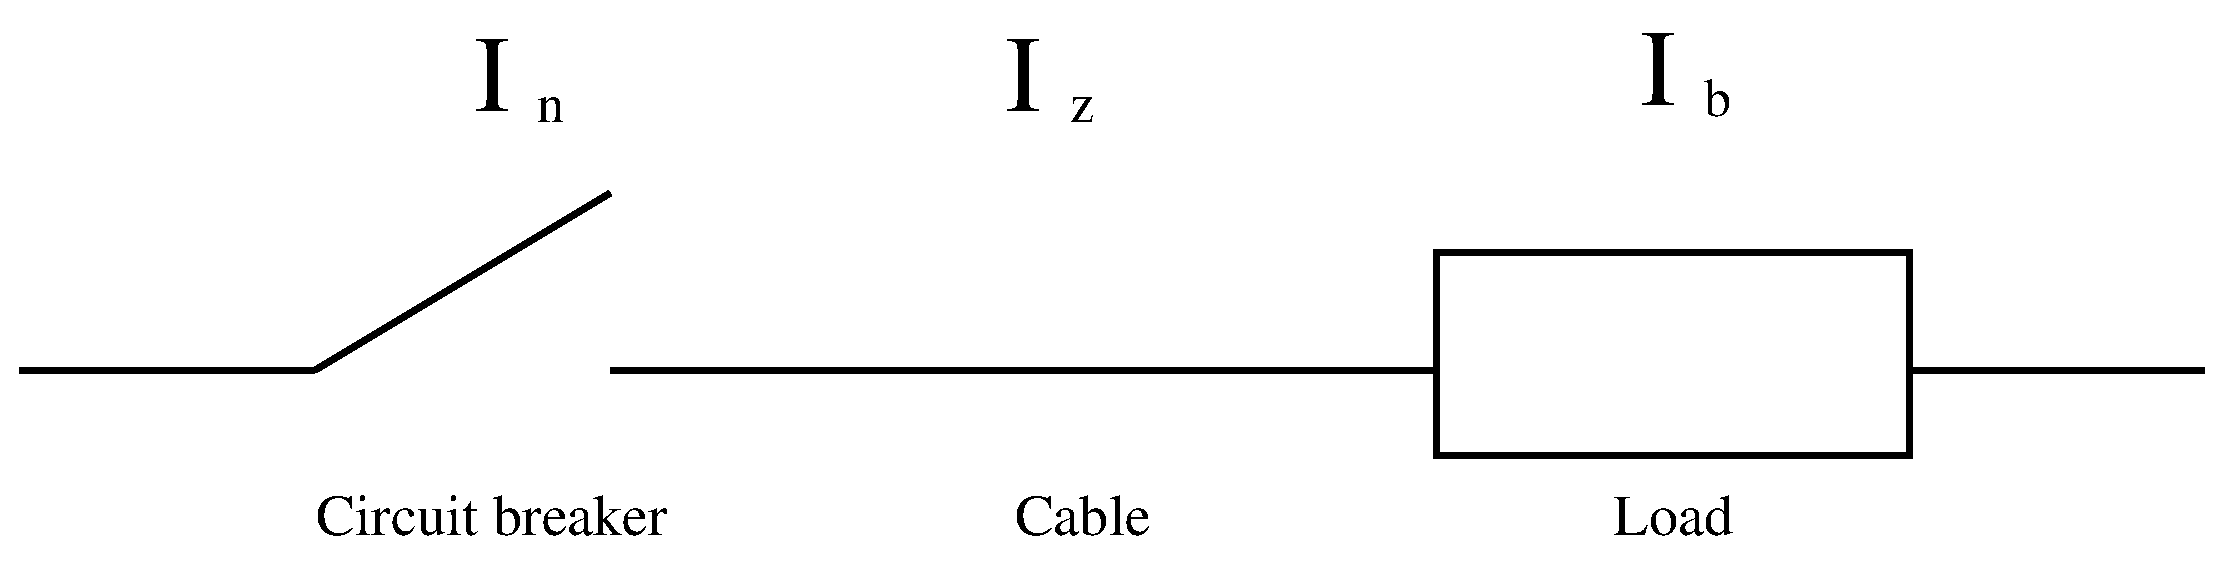
\includegraphics[width=10cm]{figures/GoldenRule.eps}
		\rule{10cm}{0.5pt} % use line???
		\caption{Graphical explanation for cable sizing.}
		\label{fig:GoldenRule}
	\end{figure}
	
	\item The simple act of writing down a new piece of information helps me to retain that knowledge better.
\end{itemize}

From these experiences, I developed a habit of keeping a time/ activity/ lesson log at my following placements for my own benefit but also in case my employers required me to submit a timesheet.
Sometimes this was the case (e.g. at Hoare Lea and Sunamp), and other times it was not (e.g. at Sweco).
A month into my placement at Sunamp, for example, I was asked to submit a timesheet.
On reflection, I am glad for my professional proactivity in keeping a log at Sunamp since they did not inform me on the timesheet requirement at the start of my placement (see log in Appendix \ref{App:Log}).



%-----------------------------------
%	SUBSECTION 2
%-----------------------------------

\subsection{Adapting to a Company's MO}

Sunamp is a unique company, unlike any other company I have worked for.
The majority of my placements have been with building design consultants, but Sunamp is a product manufacturer.
Because of their unique PCM-based products, Sunamp mixed a different set of specialists that I normally do not work with, notably salespeople, chemists, automotive and mechanical engineers, installers and production workers.
Furthermore, Sunamp was more dynamic than the companies I have worked for where the work was mostly desk-based, stationary and routinised.
At Sunamp, the people working in the office would constantly change, there were many trips between the office and the factory, and there was a general atmosphere of growth and expansion to bigger projects and new horizons.
Perhaps because Sunamp is young and fast-moving, their work processes were less routinised and their work was less accessible than what I am used to.

At my other placements, I typically had a supervisor who had drawn up a programme or list of tasks for me to carry out.
If I had a query or needed assistance, my supervisor would be my first point of contact and would most often be able to help.
Having a capable supervisor always close at hand became something that I expected at my placements.

% I encountered a stumbling block on my first day at Sunamp.

However, on my first day at Sunamp, my expectations immediately collided with their modus operandi (MO), i.e method of working.
As opposed to a clear programme or set of tasks, I was given three different job descriptions, each written by a different person.
The descriptions were unclear, vague and altogether confusing.
% In order to understand what was expected of me, I decided to speak directly with the authors of the job descriptions.
Moreover, after finding out that my main points of contact were Sandy and Joan, I learned that Sandy was usually absent but may come to the office a couple of days a week.
It turned out that Sandy's appearances were not only sparse, but also unpredictable and in high demand; everyone wanted some of Sandy's time when he was in.
This was a difficult matter for me to navigate because I had many technical questions, and he was the only person that I could address them to.
Immersed in this unfamiliar environment, I had to quickly assess Sunamp's MO and adapt to it.

% As I had been appointed to bridge the gap between Engineering and Sales (to turn technical information into meaningful information for customers), my main points of contact were Sandy (head of Engineering) and Joan (head of Sales).
% It turned out that they were the authors of two of the job descriptions.
% Carrying this expectation into Sunamp, I met my first stumbling block.

Because of the inconvenient nature of Sandy's appearances, I had to develop a tactical method to communicate with him.
When he was away, I would email him drafts of my work and request feedback.
The days he appeared in the office, I had to take a more opportunistic 
%rather than strategic
approach.
I continually updated a list of questions for Sandy so when he was ready to sit down with me, I could just grab my list and go.
But finding the time to meet with him was a bit of a challenge.
I sometimes emailed him requesting to meet him that day or the next day he was in the office.
%; this was sometimes sent as an invitation to a meeting.
Sometimes, however, he would not see the email because he was so busy in meetings or attending to other employees' needs.
During these times, I would keep an eye out for a quiet moment when he was alone and undisturbed.
I used these moments as my opportunities to notify him that I wanted to speak with him.
This opportunistic approach proved to be the most effective way to get a hold of Sandy.

\begin{comment}
Figure \ref{fig:J+S_Meetings} shows the number of meetings I managed to arrange with Joan and Sandy since my second week at Sunamp (when I had properly begun my project).
The data comes from my Sunamp log (\hl{see Appendix ...}); it is possible that I had more meetings with them than I recorded.
Overall, I had between one and three meetings a week with Joan and Sandy.
There is a decreasing trend of the number of meetings, but the main reason for this is Joan's and Sandy's absences in Weeks 4 and 6.
Considering that Joan was absent during most of Week 4 and all of Week 6, I typically met with her twice a week.
Considering that Sandy may have been absent in Week 4, I met with him on average once a week.
This shows that Joan was more readily available than Sandy.
%Don't know what else I can deduce from or reflect on this chart...


\begin{figure}[htbp]
\centering
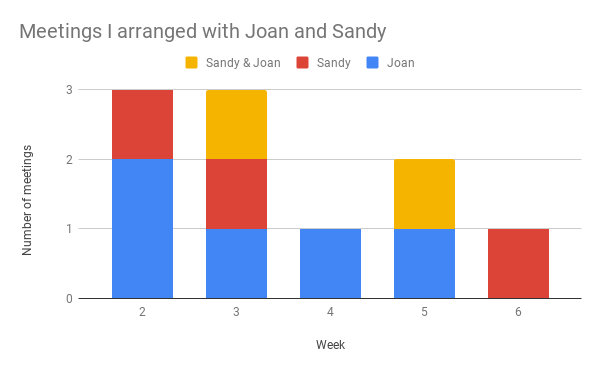
\includegraphics[width=0.7\textwidth]{figures/J+S_Meetings.png}
\rule{\textwidth}{0.5pt} % use line???
\caption{A chart displaying the number of meetings I arranged with Joan and Sandy at Sunamp.}
\label{fig:J+S_Meetings}
\end{figure}
\end{comment}

% Whereas I mostly assisted my supervisors with their projects at my other placements, the work I did at Sunamp was very much a personal project.
% ...

% I felt that Sunamp's MO was a bit disorganised.
% ...

I managed to adapt to Sunamp's MO through analysing the interpersonal relationships and responsibility hierarchy, and changing my practices to engage with it in the best way.
My ability to do this while maintaining productivity (so much so that they offered me a job at the end of the placement), demonstrate my professionalism in the workplace.




\begin{comment}
Assess very quickly some subtle and wide-ranging unique complexities that belonged to Sunamp.
They're a very unusual, different company.
I was completely immersed in their culture.
I had to change almost everything that I did to meet the way that they work/ to be able to engage with them in the way that they work.
I had to change the way that I worked, the way that I organised my time, interacted with people...
Had to either invent it or change it.
While maintaining productivity and doing it on the hoof/ every minute of the working day.
Still getting to grips with them when I left.
Did a lot at the start, and less towards the end, but always on a learning curve.
I kept my productivity up high enough that they were happy to offer me a job means that I did it right/ well.
\end{comment}

%Sunamp presentation
%\hlc[cyan]{
%	When I was preparing for my presentation, I discovered that my funnel resembles a marketing strategy/ concept called the marketing funnel.
%	This starts out by making customers aware of the product and then increasingly provides more specific information as a customer becomes more interested until they decide to purchase the product.}
%\hlc[green]{On reflection...
%	This corroborated/ validated my use of the funnel.}

%UniQ Overview Sheet
%    \hlc[green]{On reflection, the sheet misses the point of getting a heat battery. Why would I get a battery if I already have the means to generate space heating and hot water. I think this was raised during the meeting by Andrew and was to be rectified after I left.}

%Sunamp Presentation
%\hlc[cyan]{Since I gave my presentation very close to the end of my placement, I did not have time to make all the corrections and improvements that had been highlighted during the presentation.}
%\hlc[green]{On reflection, it could have been more constructive to give two presentations (first halfway through the placement and the second at the end) to allow time for me to implement their feedback.}

